\documentclass[zavrsnirad]{fer}
% Dodaj opciju upload za generiranje konačne verzije koja se učitava na FERWeb
% Add the option upload to generate the final version which is uploaded to FERWeb


\usepackage{blindtext}

\newtheorem{definition}{Definicija}
\renewcommand{\thedefinition}{\arabic{definition}.}


%--- PODACI O RADU / THESIS INFORMATION ----------------------------------------

% Naslov na engleskom jeziku / Title in English
\title{Development of an application for risk assessment in investment portfolios with the help of Monte Carlo simulations}

% Naslov na hrvatskom jeziku / Title in Croatian
\naslov{Razvoj aplikacije za procjenu rizika
u investicijskim portfeljima uz pomoć Monte Carlo simulacija}

% Broj rada / Thesis number
\brojrada{1951}

% Autor / Author
\author{Ivan Džanija}

% Mentor
\mentor{Prof.\@ Mihaela Vranić}

% Datum rada na engleskom jeziku / Date in English
\date{June, 2025}

% Datum rada na hrvatskom jeziku / Date in Croatian
\datum{lipanj, 2025.}

%-------------------------------------------------------------------------------


\begin{document}

% Naslovnica se automatski generira / Titlepage is automatically generated
\maketitle

%--- ZADATAK / THESIS ASSIGNMENT -----------------------------------------------

% Zadatak se ubacuje iz vanjske datoteke / Thesis assignment is included from external file
% Upiši ime PDF datoteke preuzete s FERWeb-a / Enter the filename of the PDF downloaded from FERWeb
\zadatak{zadatak.pdf}

%--- ZAHVALE / ACKNOWLEDGMENT --------------------------------------------------

\begin{zahvale}
	% Ovdje upišite zahvale / Write in the acknowledgment
	Hvala na svemu puno.
	ovo je test i opet
\end{zahvale}

% Odovud započinje numeriranje stranica / Page numbering starts from here
\mainmatter

% Sadržaj se automatski generira / Table of contents is automatically generated
\tableofcontents

%--- UVOD / INTRODUCTION -------------------------------------------------------
\chapter{Uvod}
\label{pog:uvod}

Modeliranje ponašanja portfelja je jedna od ključnih metoda pri odabiru
investicijskih ulaganja ili sigurnih financijskih rezervi.

Neki od radova koje ćemo citirati su \cite{1,2,6248073,6247753,ghiglia_pritt_phase_unwrapping,4250461}.
Trebaju nam samo radi testiranja kako izgleda referenciranje rada s konferencije, rada iz časopisa, knjige i Internetske stranice.

\begin{figure}[htb]
	\centering
	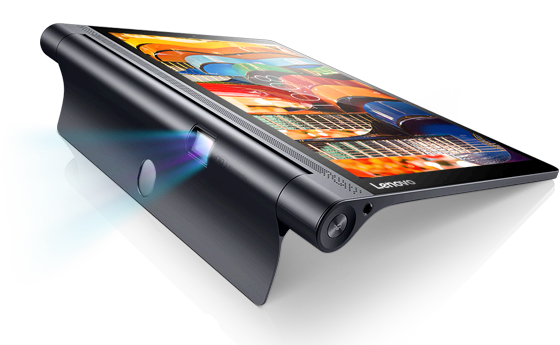
\includegraphics[width=0.38\linewidth]{Figures/lenovo_yoga_tab3_pro_front.png}
	\caption{Moja prva slika}
	\label{slk:prvaslika}
\end{figure}

Referenciramo se na sliku \ref{slk:prvaslika} u sredini rečenice, zatim prije zareza \ref{slk:prvaslika}, te zatim na kraju rečenice \ref{slk:prvaslika}.
Upravo smo testirali radi li naredba \verb|\ref| ispravno u slučaju kada nakon nje slijedi točka.

Sada slijedi jedna jednadžba:
\begin{equation}
	\label{jed:prvajednadzba}
	\int_{-\infty}^{+\infty}f(t)\,dt=F(\omega)
\end{equation}
Jednadžba \eqref{jed:prvajednadzba} je moja prva jednadžba koja defnira par $f(t)\ufrek F(\omega)$ ili $F(\omega)\uvrem f(t)$.

%-------------------------------------------------------------------------------
\chapter{Teorija portfelja}
\label{pog:teorija_portelja}

Teorija portfelja daje strogu matematičku definiciju
financijskim pojmovima i predstavlja temelj matematičnog
modeliranja investicija i drugih financijskih instrumenata.
Trebam navesti jos zacetnika i pocetak teorije portfelja te formulirati
optimizacijski problem -> povecanje povrata i smanjenje rizika

\section{Povrati}
\label{sek:povrati}

Povrat definiramo kao postotnu promjene cijene financijskog
instrumenta kroz određeni vremenski period.

\begin{definition}
	Neka je $P_t$ cijena financijskog instrumenta u trenutku $t$ te
	$P_0$ početna cijena istog instrumenta. Povrat $R_t$ definiramo kao:
\end{definition}
\begin{align*}R_t = \frac{P_t}{P_0} - 1 = \frac{P_t - P_0}{P_0}
\end{align*}

\noindent Neka buduća cijena nam neće biti poznata pri investiranju te zato povrat promatramo kao slučajnu varijablu.
Vidimo kako je moguće imati negativan povrat ako je cijena koju promatramo
manja od početne cijene i to je upravo situacija koji pokušavamo izbjeći.
\begin{definition}
	Očekivani povrat promatramo kao srednju vrijednost prijašnjih
	povrata jer je upravo srednja vrijednost nepristran procjenitelj
	očekivanja slučajne varijable $R_t$ za koji vrijedi:
\end{definition}
\begin{align*}
	E(R_t) =\frac{1}{N} \sum_{i = 1}^{N} R_i
\end{align*}

\section{Volatilnost}
Drugi dio optimizacijskog problema teorije portfelja je smanjenje rizika.
Volatilnost je upravo jednostavna mjera rizika koja ima pogodna matematička svojstva.
Promatramo je kao standardnu devijaciju slučajne varijable $R_t$, a ima je smisla tako promatrati
jer će nam upravo takva mjera kvantificirati kretanje povrata.
\begin{definition}
	Volatilnost investicije definiramo kao nepristran procjenitelj
	standardne devijacije slučajne varijable $R_t$:
\end{definition}
\begin{align*}
	\sigma_R = \sqrt{\frac{1}{N - 1} \sum_{i = 1}^{N} \left[R_i - E(R_t)\right]^2}
\end{align*}
\\
Kod ovakvog jednostavnog modela rizika imamo problem što jednako tretiramo i pozitivane i negativne povrate.
U slučajevima kada modeliramo kretanje povrata sa simetričnom distribucijom ovo
ne mora biti problem, ali to nije uvijek slučaj.

\section{Portfelj}
Investicijske portfelje matematički prikazujemo kao linearnu kombinaciju
pojedinih investicija sa vektorom pojedinih udjela $\mathbf{w}$.
\begin{definition}
	Vektor $\mathbf{w}$ predstavlja udjele investicija u portfelju.
\end{definition}
\begin{align*}
	\mathbf{w} = \begin{pmatrix} w_1 \\ w_2 \\ ... \\ w_N \end{pmatrix},
	\indent \sum_{i = 1}^{N} w_i = 1
\end{align*}

\begin{definition}
	Povrat portfelja je ponderirani prosjek povrata investicija u portfelju:
\end{definition}
\begin{align*}
	R_p = \sum_{i = 1}^{N} w_i R_i
\end{align*}
\indent Vidimo kako je povrat portfelja zapravo otežana suma povrata svih investicija.

\begin{definition}
	Volatilnost portfelja definiramo:
\end{definition}
\begin{align*}
	\sqrt{Var(R_p)} = \sqrt{\mathbf{w^\intercal}\boldsymbol{\Sigma} \mathbf{w}} \\
\end{align*}
\indent \quad \quad $\mathbf{w}$ je ranije definirani vektor udjela investicija\\
\indent \quad \quad $\boldsymbol{\Sigma}$ je matrica kovarijance slučajnog vektora $\mathbf{w}$\\


% Rasprava
\chapter{Rezultati i rasprava}
\label{pog:rezultati_i_rasprava}

\Blindtext

%--- ZAKLJUČAK / CONCLUSION ----------------------------------------------------
\chapter{Zaključak}
\label{pog:zakljucak}

\blindtext

%--- LITERATURA / REFERENCES ---------------------------------------------------

% Literatura se automatski generira iz zadane .bib datoteke / References are automatically generated from the supplied .bib file
% Upiši ime BibTeX datoteke bez .bib nastavka / Enter the name of the BibTeX file without .bib extension
\bibliography{literatura}

%--- SAŽETAK / ABSTRACT --------------------------------------------------------

% Sažetak na hrvatskom
\begin{sazetak}
	Unesite sažetak na hrvatskom.

	\blindtext
\end{sazetak}

\begin{kljucnerijeci}
	prva ključna riječ; druga ključna riječ; treća ključna riječ
\end{kljucnerijeci}

% Abstract in English
\begin{abstract}
	Enter the abstract in English.

	\blindtext
\end{abstract}

\begin{keywords}
	the first keyword; the second keyword; the third keyword
\end{keywords}

%--- PRIVITCI / APPENDIX -------------------------------------------------------

% Sva poglavlja koja slijede će biti označena slovom i riječi privitak / All following chapters will be denoted with an appendix and a letter
\backmatter

\chapter{The Code}

\Blindtext

\end{document}
